\begin{egBox}{Completely Regular Spaces}[eg:33.1]
    Normal spaces are completely regular.
\end{egBox}

\begin{egBox}{Illustration of Step 1 in the [\hyperlink{thm:33.1}{Urysohn Lemma}] \ 
    Proof}[eg:33.2]
    Let us suppose we started with the standard way of arranging the elements of \( P \)
    in an infinite sequence:
    \begin{equation*}
        P
        =
        \left\{
            0, 1, \frac{ 1 }{ 2 }, \frac{ 1 }{ 3 }, \frac{ 2 }{ 3 },
            \frac{ 1 }{ 4 }, \frac{ 3 }{ 4 }, \frac{ 1 }{ 5 }, \frac{ 2 }{ 5 },
            \frac{ 3 }{ 5 }, \ldots
        \right\}
    \end{equation*}
    After defining \( U_{ 0 } \) and \( U_{ 1 } \) as done in the proof, we would
    define \( U_{ \frac{ 1 }{ 2 } } \) (using the normality of \( X \)) so that 
    \begin{equation*}
        \overline{ U_{ 0 } } \subset U_{ \frac{ 1 }{ 2 } }
        \quad \mathrm{and} \quad 
        \overline{ U_{ \frac{ 1 }{ 2 } } } \subset U_{ 1 }
    \end{equation*}
    Then, we would fit \( U_{ \frac{ 1 }{ 3 } } \) in between \( U_{ 0 } \) and 
    \( U_{ \frac{ 1 }{ 3 } } \) so that 
    \begin{equation*}
        \overline{ U_{ 0 } } \subset U_{ \frac{ 1 }{ 3 } }
        \quad \mathrm{and} \quad 
        \overline{ U_{ \frac{ 1 }{ 3 } } } \subset U_{ \frac{ 1 }{ 2 } }
    \end{equation*}
    Then, we would fit \( U_{ \frac{ 2 }{ 3 } } \) in between 
    \( U_{ \frac{ 1 }{ 2 } } \) and \( U_{ 1 } \) so that 
    \begin{equation*}
        \overline{ U_{ \frac{ 1 }{ 2 } } } \subset U_{ \frac{ 2 }{ 3 } }
        \quad \mathrm{and} \quad 
        \overline{ U_{ \frac{ 2 }{ 3 } } } \subset U_{ 1 }
    \end{equation*}
    And so on.

    \begin{figure}[H]
        \centering
        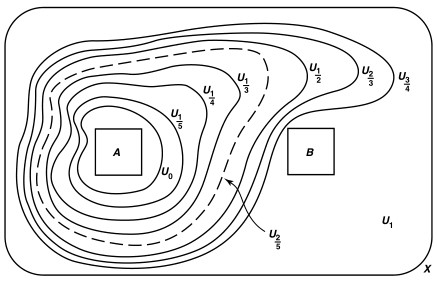
\includegraphics[ width = 0.6\linewidth ]{figures/Section 33/eg33-2.jpg}
        \caption{An Illustration of Step 1 in the Urysohn Lemma}
        \label{fig:33-1}
    \end{figure}
\end{egBox}